\begin{figure}[!htbp]
\centering
\begin{subfigure}[b]{0.5\textwidth}
    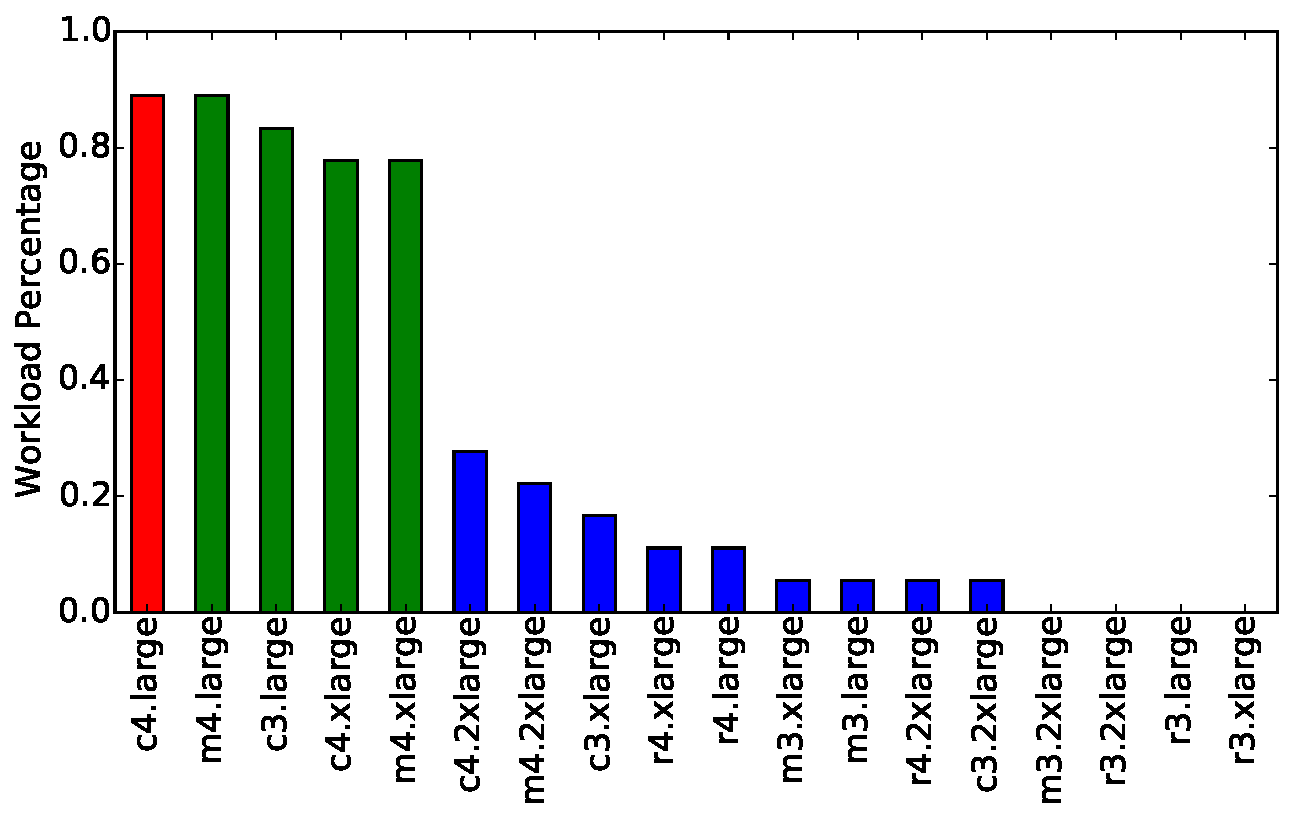
\includegraphics[width=\linewidth]{Figures/motivation_cost_hadoop_percentage.pdf}
    \caption{Hadoop 2.7}
    \label{fig:motivation_percentage_1}
\end{subfigure}
\begin{subfigure}[b]{0.5\textwidth}
    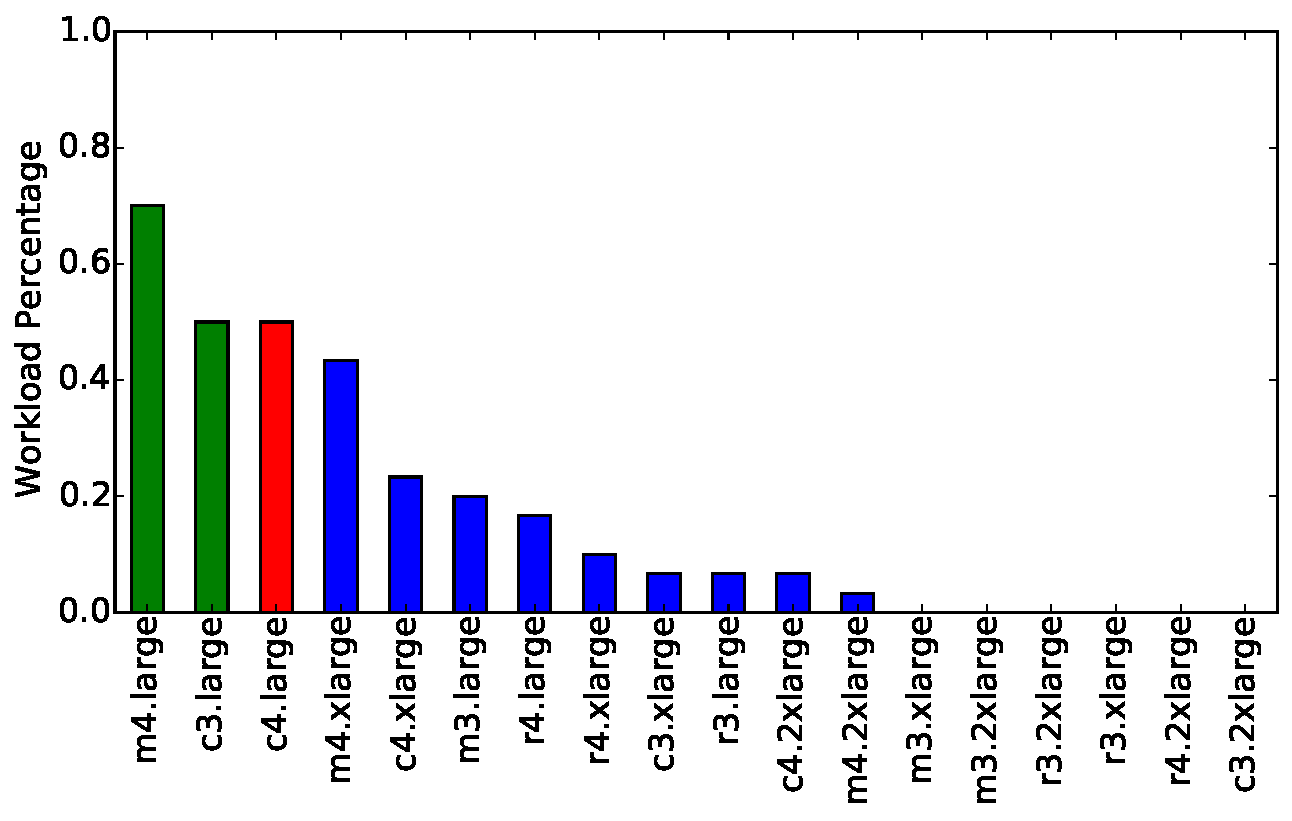
\includegraphics[width=\linewidth]{Figures/motivation_cost_spark_percentage.pdf}
    \caption{Spark 2.1}
    \label{fig:motivation_percentage_2}
\end{subfigure}
\begin{subfigure}[b]{0.5\textwidth}
    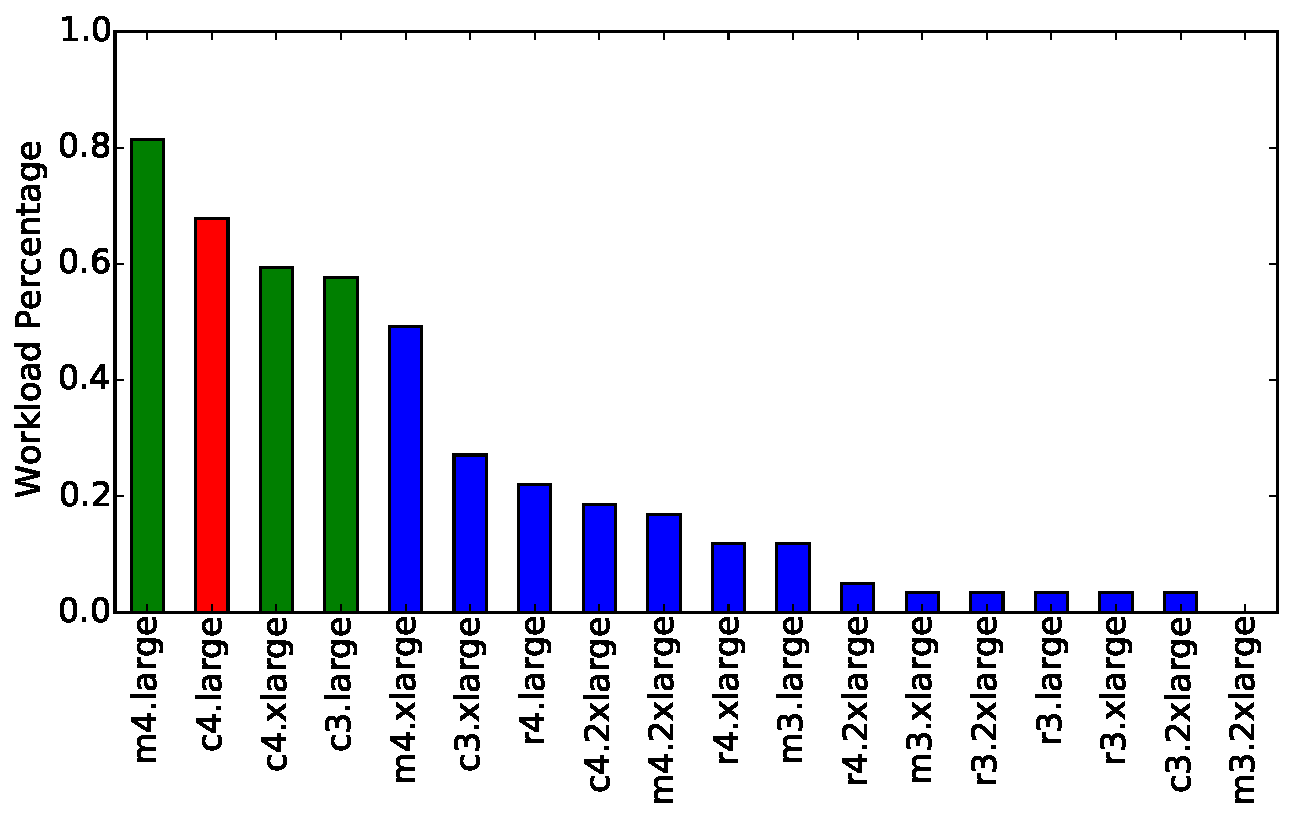
\includegraphics[width=\linewidth]{Figures/motivation_cost_spark1.5_percentage.pdf}
    \caption{Spark 1.5}
    \label{fig:motivation_percentage_3}
\end{subfigure}
\caption{\textbf{Opportunity to find the exemplar VM instances across workloads for reducing operational cost.} The \emph{y-axis} represents the percentage of workloads (out of 107 in three systems) that are within 30\% difference with the optimal performance.  The colored bars are VM types that considered the exemplar configurations for the majority of workloads ($>= 50\%$).
 The \textcolor{red}{red} bar represents that the VM type is more likely to be the optimal choice.}
\label{fig:motivation_percentage}
\end{figure}


\section{Finding the Exemplar Cloud Configuration}
\label{sec:mab}

In this section, we first present our empirical study
on investigating the potential of finding the exemplar cloud configuration.
We then formulate ``finding the exemplar configuration in the cloud'' as the multi-armed bandit problem.
Finally, we discuss the heuristics to derive the exemplar configuration.

%\todo{we can extend to find multiple exemplar configurations}


\subsection{Empirical Study}
\label{sec:empirical}

We choose three popular software systems for cloud applications, namely Apache Hadoop 2.7, Spark 2.1 and Spark 1.5.
This study includes 30 applications for diversification.
They are data processing, OLAP queries, common statistics functions, and
popular machine learning algorithms.
Although they do not cover all the spectrum of real-world applications,
they are representative of many nowadays cloud applications.
When the input to applications changes, the workload behavior changes accordingly~\cite{Venkataraman2016, Dalibard2017}.
We also choose three different input parameters and data sizes for each application.
In total, our evaluation includes 107 workloads.

We conduct our evaluation on AWS EC2~\cite{aws}.
Regarding the VM to run the workloads, we choose 18 different VM types.
They include three instance families:
1) compute-optimized instances (\emph{c3} and \emph{c4}),
2) memory-optimized instances (\emph{r3} and \emph{r4}), and
3) general-purpose instances (\emph{m3} and \emph{m4}).
For each instance family, we choose \emph{large}, \emph{xlarge} and \emph{2xlarge} for the instance size.
Although we only evaluate 21\% VM types (AWS supports 85 kinds as of January in 2018),
they reflect many use cases on AWS EC2.
Besides, some VM types are designed for acceleration using GPU and FPGA, and therefore, they are less common and not included.
Furthermore, it is reported that VM types with lower than 8 cores dominate VM useage on Azure~\cite{Cortez2017}.
We try our best to reflect the common cloud deployment.
More details regrading data collection can be found in our previous work~\cite{Hsu2018Arrow, Hsu2018Scout}.
We also made our data public available for further research~\cite{scoutdataset}.
Please refer Section~\ref{sec:cat::dataset} in more detail.



\subsection{The Exemplar Configurations}
\label{sec:exemplar}
The exemplar configurations are configurations that
are near-optimal or satisfactory in the majority of workloads.
When the percentage is large, 
we can exploit the exemplar configurations to simplify collective optimization.
In \myfigure{\ref{fig:motivation_percentage}}, we present the opportunity of exploiting such configurations.
We count the number of the normalized performance that is within 30\% of the optimal.
The colored bars are possible exemplars because they are satisfactory at least in half of the workloads.
The red bar represents the VM type that is more likely to be the optimal than other configurations.
These figures show there exist several exemplar configurations.


% % datasize=medium
\begin{table}[!htbp]
\centering
\caption{\textbf{Normalized performance on a selected group of VM types and workloads.}  The number $1.0$ represents the optimal choice across the 18 VM types for the particular workload.}
\label{table:dataset}
%{\scriptsize
\resizebox{0.75\columnwidth}{!}{%
\renewcommand{\baselinestretch}{0.5} 
\begin{tabular}{@{}c@{~}l@{~}r@{~}r@{~}r@{~}r@{~}r@{}}
\toprule
\multicolumn{1}{l}{\textbf{System}} & \textbf{Workload} & \textbf{c3.large} & \textbf{c4.large} & \textbf{c4.xlarge} & \textbf{m4.large} & \textbf{m4.xlarge} \\ \midrule
\multirow{6}{*}{\rotatebox[origin=c]{90}{\parbox[c]{1.5cm}{\centering Hadoop 2.7}}} & aggregation & 1.26 & 1.00 & 1.12 & 1.12 & 1.29 \\
 & join & 1.26 & 1.00 & 1.09 & 1.17 & 1.26 \\
 & scan & 1.16 & 1.00 & 1.70 & 1.15 & 1.89 \\
 & sort & 1.10 & 1.00 & 1.06 & 1.03 & 1.11 \\
 & terasort & 1.31 & 1.00 & 1.16 & 1.07 & 1.12 \\
 & pagerank & 1.24 & 1.03 & 1.16 & 1.05 & 1.00 \\ \midrule
\multirow{10}{*}{\rotatebox[origin=c]{90}{\parbox[c]{1cm}{\centering Spark 2.2}}} & join & 1.12 & 1.00 & 1.40 & 1.12 & 1.23 \\
 & scan & 1.13 & 1.00 & 1.48 & 1.03 & 1.59 \\
 & sort & 1.11 & 1.00 & 1.42 & 1.13 & 1.40 \\
 & terasort & 1.30 & 1.19 & 1.66 & 1.34 & 1.46 \\
 & wordcount & 1.83 & 1.64 & 1.23 & 1.00 & 1.08 \\
 & als & 1.00 & 1.67 & 3.19 & 1.46 & 2.72 \\
 & aggregation & 1.30 & 2.00 & 1.08 & 1.00 & 1.18 \\
 & pagerank & 2.33 & 2.12 & 1.00 & 1.31 & 2.10 \\
 & bayes & 3.15 & 3.57 & 1.00 & 1.60 & 1.61 \\
 & lr & 6.50 & 5.56 & 1.44 & 1.00 & 2.61 \\ \midrule
\multirow{19}{*}{\rotatebox[origin=c]{90}{\parbox[c]{1cm}{\centering Spark 1.5}}} & chi-feature & 1.19 & 1.00 & 1.32 & 1.29 & 1.53 \\
 & fp-growth & 1.27 & 1.00 & 1.37 & 1.20 & 1.46 \\
 & gmm & 1.19 & 1.00 & 1.27 & 1.25 & 1.36 \\
 & gb-tree & 1.19 & 1.00 & 1.63 & 1.17 & 1.94 \\
 & pca & 1.16 & 1.00 & 1.11 & 1.15 & 1.31 \\
 & pearson & 1.19 & 1.00 & 1.11 & 1.19 & 1.11 \\
 & word2vec & 1.22 & 1.00 & 1.06 & 1.15 & 1.24 \\
 & spearman & 1.21 & 1.00 & 1.12 & 1.06 & 1.02 \\
 & statistics & 1.15 & 1.00 & 1.43 & 1.08 & 1.56 \\
 & svd & 1.16 & 1.00 & 1.02 & 1.07 & 1.09 \\
 & chi-gof & 1.24 & 1.12 & 1.46 & 1.00 & 1.81 \\
 & bayes & 1.27 & 1.15 & 1.19 & 1.25 & 1.35 \\
 & lda & 1.66 & 1.36 & 1.10 & 1.00 & 1.31 \\
 & pic & 1.53 & 1.39 & 1.00 & 1.15 & 1.31 \\
 & d-tree & 1.70 & 1.70 & 1.23 & 1.00 & 1.48 \\
 & als & 2.23 & 1.86 & 2.89 & 1.00 & 1.27 \\
 & regression & 4.03 & 3.60 & 4.06 & 4.42 & 4.70 \\
 & classification & 6.11 & 5.41 & 5.70 & 6.07 & 1.00 \\
 & kmeans & 6.22 & 5.74 & 3.66 & 3.73 & 1.00 \\ \midrule
\multicolumn{2}{c}{\textbf{\# of optimal}} & 1 & 18 & 3 & 7 & 3 \\
\multicolumn{2}{c}{\textbf{Mean}} & 1.89 & 1.72 & 1.63 & \textbf{1.45} & 1.53 \\
\multicolumn{2}{c}{\textbf{25\%}} & 1.18 & 1.00 & 1.11 & 1.04 & 1.15 \\
\multicolumn{2}{c}{\textbf{Median}} & 1.26 & 1.00 & 1.23 & 1.15 & 1.31 \\
\multicolumn{2}{c}{\textbf{75\%}} & 1.68 & 1.69 & 1.47 & \textbf{1.25} & 1.58 \\ \bottomrule
\end{tabular}
}
\end{table}


In \mytable{\ref{table:dataset}}, we give snippets of measurement data to better illustrate the exemplar configurations.
This table presents the normalized performance of workloads on some of the VM types.
A $1.0$ number indicates the VM type is the optimal choice for the corresponding workload while a larger number implies a sub-optimal choice.
We can observe that \emph{c4.large} is the optimal configuration for 18 workloads (out of 35).
However, it is also a sub-optimal VM type ($>1.4$) in 11 workloads, which generating
$1.72$ normalized performance on average.
On the other hand, \emph{m4.large} seems to be a better choice because it delivers $1.45$ performance on average and creates only 5 sub-optimal workloads.
The above gives one way to select the exemplar configuration and in the following,
we describe the challenges of selecting the exemplar.



\begin{itemize}
\item \textbf{Varying workloads.}
In \mytable{\ref{table:dataset}}, we show five possible exemplar configurations for those particular workloads.
The exemplars very in different sets of workloads.
For example, \emph{c4.large} is the best choice in Hadoop 2.7 while
\emph{m4.large} should be selected as the exemplar VM type in Spark 2.1.

\item \textbf{Expanding cloud portfolio.}
As mentioned before, cloud providers introduce new VM types regularly, which
includes performance boost and price adjustment.
The exemplar configurations might also change accordingly.

\item \textbf{Online discovery.}
We present an offline analysis of measurement data above.
However, finding the exemplar configuration is an online task (for unknown workloads), which is considered a difficult learning problem.
This is similar to the exploration-exploitation dilemma~\cite{kaelbling1996reinforcement}.

\end{itemize}

From the above, it would appear that there exist exemplar configurations in real-world workloads.
Note that if the exemplar configuration is prevalent, it should be possible to simplify collective optimization as follows:
finding the exemplar configuration instead of finding the optimal choice for each of the workload.
The exemplar configurations deliver near-optimal to satisfactory performance in the majority of workloads.
The rest of this work is a test of that speculation.






\subsection{Problem Formulation}
\label{sec:formulation}

\micky attempts to find the exemplar VM type ($vm^*\in VM$) for a group of workloads ($W$).
The workload refers to a combination of an application and the data used.
The performance is measured in terms of \textit{execution time} and \textit{operational cost}. The cloud configuration space for workload
$w$ is referred to as ($s\in S_w$), where $S_w$ is the set of cloud configuration options for a workload $w$. The size
of the search space is $N_w$ cloud configurations. In our setting, the size of the cloud configuration space is same for all workloads. For a given workload $w$, each configuration $s$ has a corresponding performance
measure $y_{w, s} = \phi(w, s)$.
%Each configuration in the cloud configuration space $s$ is represented as the features of the cloud configuration such as number of cores, size of the memory.
%The objective is to find a cloud

Single-optimizers such as Cherrypick~\cite{Alipourfard2017} searches a suitable VM type for every workload $w$ separately.
The search starts with a pool of unevaluated configuration ($U_w$)---the specific workload has not been run on any configuration.
As the search proceeds, the cloud configuration are selected from $U_w$ and moved to the evaluated pool ($E_w$). The sum of the cardinalities
of $U_w$ and $E_w$ is equal to the cardinality of $S_w$ ($|U_w| +|E_w| = |S_w|$).
The measurement cost of the search process is $C_w=|E_w|$.
When optimizing a group of workloads,
single-optimizers generate a total cost $C=\sum_{w \in W} |C_w|$.

\micky is a collective optimization method.
We explore the exemplar VM type $vm^*$ so that 
$|E_{w_1} \cup E_{w_2} \cup \cdots \cup E_{w_n}|$ is minimized while the corresponding performance measure
$y_{w, vm^*}$ is comparable to the the ones in single-optimizers.



\subsection{The Multi-Armed Bandit Problem}

To realize collective optimization, we reformulate the problem of configuration optimization as a multi-armed bandit problem~
\cite{robbins1985some,weber1992gittins,bergemann2006bandit,audibert2011introduction}.
In the problem setting,
an agent  (gambler) sequentially searches for a slot machine (from a group of slot machines) to maximize the total reward collected in the long run. This problem is non-trivial since the agent (gambler) cannot access the true probability of winning---all learning is carried out via the means of trial-and-error and value estimation. To find the suitable slot machine, the agent needs to acquire information about arms  (exploration)  while  simultaneously  optimizing  immediate rewards  (exploitation).
The is referred to as the exploration-exploitation dilemma~\cite{kaelbling1996reinforcement}.
Finding the better VM type for workloads naturally fits into the multi-armed bandit problem.
We describe their similarities in the following.

\begin{itemize}
\item \textbf{Slot Machine.} Each VM type is similar to a slot machine. Our objective is to find the best VM that maximizes the reward for a group of workloads.
\item \textbf{Arm.} Arms are the choices of slot machines. In the cloud setting, an optimizer chooses a VM type to run a workload.
\item \textbf{Pull.} A pull is one play on the slot machine. It takes coins (cost) and yields a reward.
Similarly, an optimizer picks a VM type and measures the performance of a workload on the selected VM.
\item \textbf{Reward.} Reward refers to the amount of money a gambler wins or loses from pulling the arms.
In our setting, the reward is determined by where it meets a performance objective.
We use performance delta (between the selected and the optimal choice) for calculating the reward.
Please note that the optimal configuration is not known in the real-world setting.
\item \textbf{Budget.}
A gambler owns a certain amount to spend on the slot machines.
In our setting, an optimizer requires to complete the optimization process in a limited budget.
We use the number of measurements as the budget ($C$).
In practice, the minimal budget is usually $|\mathit{VM}|$
and the maximum budget is $|\mathit{VM}| \times |\mathit{W}|$.
The budget is determined by users.
A higher budget yields a better reward.
\item \textbf{Objective.}
The objective of \micky is to find the best configuration (minimize performance delta) for multiple workloads with fewer measurements.
\end{itemize}

The multi-armed bandit problems have attracted attention for solving online learning problems.
For example, 
Dambreville et al.~\cite{dambreville2017load} used multi-arm bandit to minimize the energy consumption of a cloud platform by
using workload prediction to reallocate the set of available servers.
Jiang et al. perform data-driven QoE (quality of experience) optimization for real-time exploration and exploitation~\cite{jiang2017pytheas}.
While we borrow techniques from this rich literature~\cite{bergemann2006bandit}, our contribution is to shed light on how to use these techniques to find the exemplar cloud configurations and to show collective optimization can solve the problem using only a fraction of measurement cost required by prior work.


\begin{figure}[!htbp]
\centering
\begin{subfigure}[b]{0.6\textwidth}
    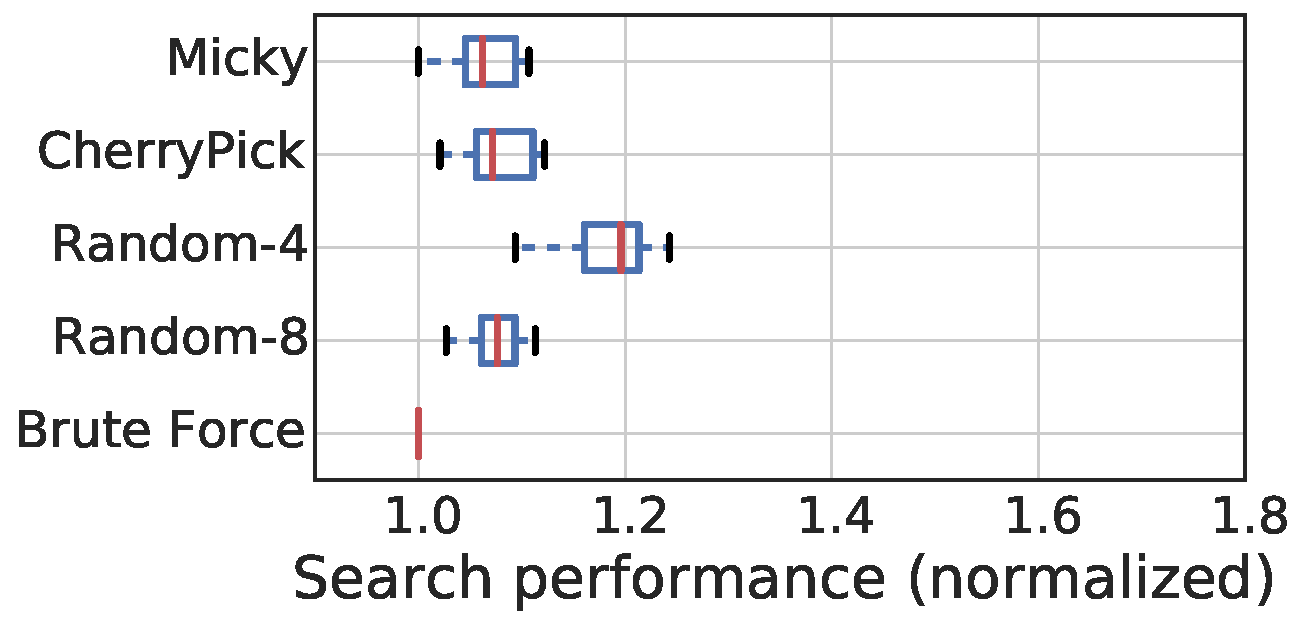
\includegraphics[width=\linewidth]{Figures/s2_single_hadoop_cost_performance.pdf}
    \caption{Hadoop 2.7}
    \label{fig:single_time_steps}
\end{subfigure}
\begin{subfigure}[b]{0.6\textwidth}
    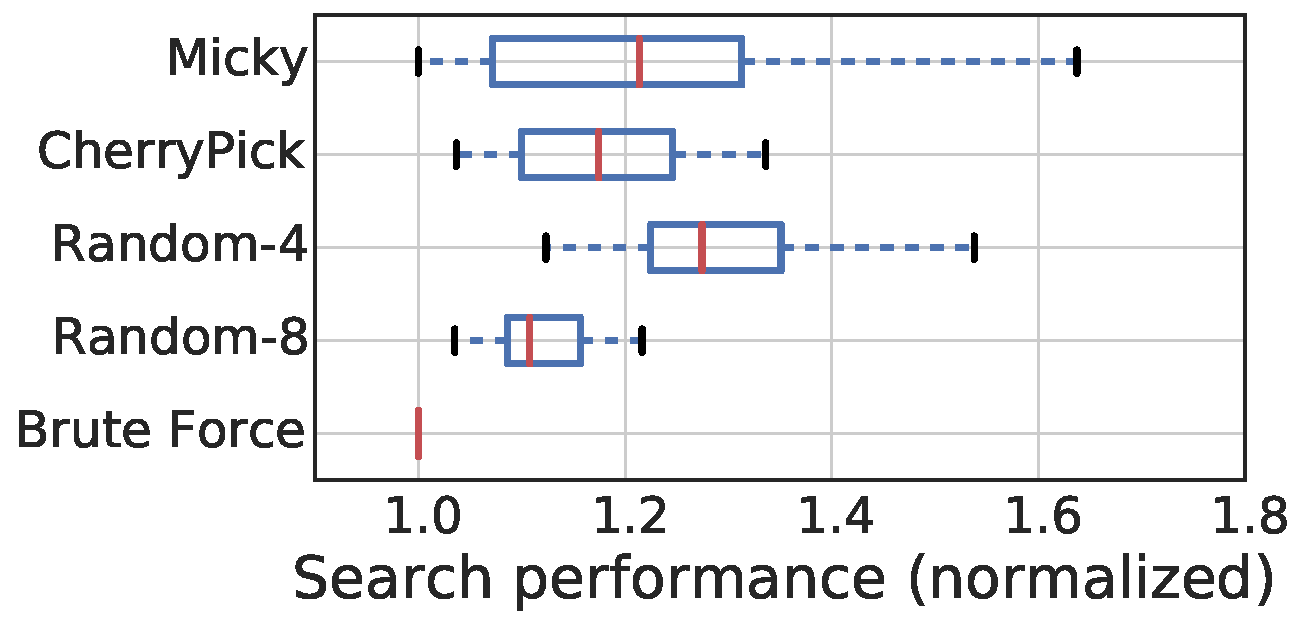
\includegraphics[width=\linewidth]{Figures/s2_single_spark_cost_performance.pdf}
    \caption{Spark 2.1}
    \label{fig:single_time_performance}
\end{subfigure}
\begin{subfigure}[b]{0.6\textwidth}
    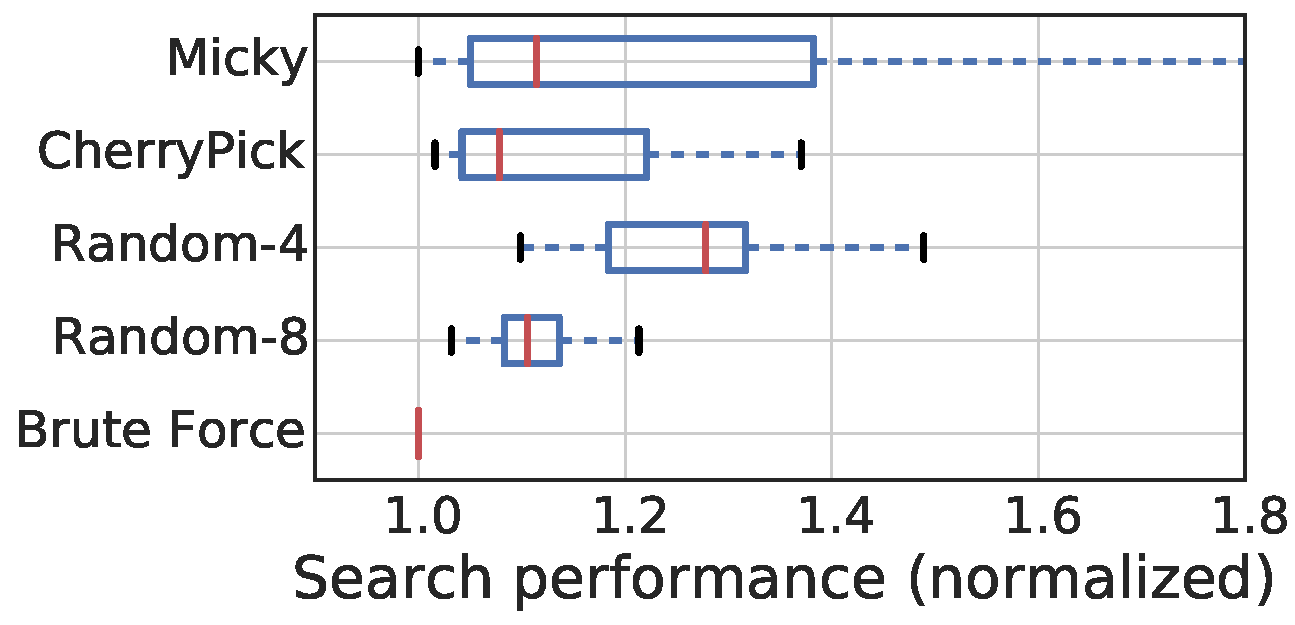
\includegraphics[width=\linewidth]{Figures/s2_single_spark15_cost_performance.pdf}
    \caption{Spark 1.5}
    \label{fig:single_time_performance}
\end{subfigure}
\caption{\small{\textbf{Search performance of optimization methods in search for cost-effective cloud configurations.} Three software systems are evaluated.  \emph{CherryPick} finds good solutions in the three systems while \micky is comparable in Hadoop 2.7 but shows higher variance (sub-optimal choices).  We propose a integrated system (in \myfigure{\ref{fig:system_design}}) to detect those sub-optimal cases for improving \micky.}}
\label{fig:s2_cost_performance}
\end{figure}


\subsection{Heuristics}
\label{sec:methods}

% need to put softmax in the following text
% we might need to try thompson sampling
% need citation
In the literature, several strategies have been proposed to find the most rewarding slot machines (the exemplar configurations) in the multi-arm bandit setting.
These strategies can be divided into three major groups.
First, the \textit{Epsilon-greedy}, works by oscillating between (a) exploiting the best option which is currently known, and (b) exploring at random among all of the options available to it.
Second, the probability matching strategy selects the arms according to the probability of the arm being the optimal choice.
Thompson sampling or Bayesian Bandits are well-known probability matching strategies.
Last, in the contextual bandit problem, strategies such as Upper Confidence Bound (UCB) builds a predictor from existing observation for making a better decision.
UCB always opportunistically chooses the arm that has the highest upper confidence bound of reward, and therefore, it will naturally tend to use arms with high
expected rewards or high uncertainty.
The above only discusses some important methods.
It is not the major focus to design the best method but to evaluate the existing methods best for collective optimization.